\documentclass[12pt,oneside,letterpaper]{article}
\usepackage{listings}
\usepackage{color}
\usepackage{mathtools}
\usepackage{graphicx}
\usepackage{fontspec}

\definecolor{background}{RGB}{39, 40, 34}
\definecolor{string}{RGB}{230, 219, 116}
\definecolor{comment}{RGB}{117, 113, 94}
\definecolor{normal}{RGB}{248, 248, 242}
\definecolor{identifier}{RGB}{166, 226, 46}
\setmonofont{Consolas}
% \usepackage{babel}
% \usepackage{blindtext}
\title{	ECE3849 Lab 2}
\author{Nam Tran Ngoc\\
		Yigit Yuan\\
    Mailbox 388}

\lstset{
  language=C,                      % choose the language of the code
  numbers=left,                       % where to put the line-numbers
  stepnumber=1,                       % the step between two line-numbers.        
  numbersep=5pt,                      % how far the line-numbers are from the code
  numberstyle=\tiny\color{black}\ttfamily,
  backgroundcolor=\color{background},     % choose the background color. You must add \usepackage{color}
  showspaces=false,                   % show spaces adding particular underscores
  showstringspaces=false,             % underline spaces within strings
  showtabs=false,                     % show tabs within strings adding particular underscores
  tabsize=4,                          % sets default tabsize to 2 spaces
  captionpos=b,                       % sets the caption-position to bottom
  breaklines=true,                    % sets automatic line breaking
  breakatwhitespace=true,             % sets if automatic breaks should only happen at whitespace
  title=\lstname,                     % show the filename of files included with \lstinputlisting;
  basicstyle=\color{normal}\ttfamily,         % sets font style for the code
  keywordstyle=\color{magenta}\ttfamily,  % sets color for keywords
  stringstyle=\color{string}\ttfamily,    % sets color for strings
  commentstyle=\color{comment}\ttfamily,  % sets color for comments
  emph={Semaphore_pend, Semaphore_post, Mailbox_pend, Mailbox_post, main},
  emphstyle=\color{identifier}\ttfamily
}

\begin{document}
\maketitle
\cleardoublepage
\section{Introduction}
Our previous assignment was to build a real-time digital oscilloscope that is capable to gather 500.000 samples each second and display the signal on the built in display. In this lab, we take this a step further by implementing the same features using TI’s SYS/BIOS Real Time Operating System (RTOS). We created various tasks and RTOS objects to mimic the foreground - background system from the previous lab. Furthermore, we integrated the Kiss FFT package to compute and display the spectrum of the sampled signal. 

\begin{figure}[h]
  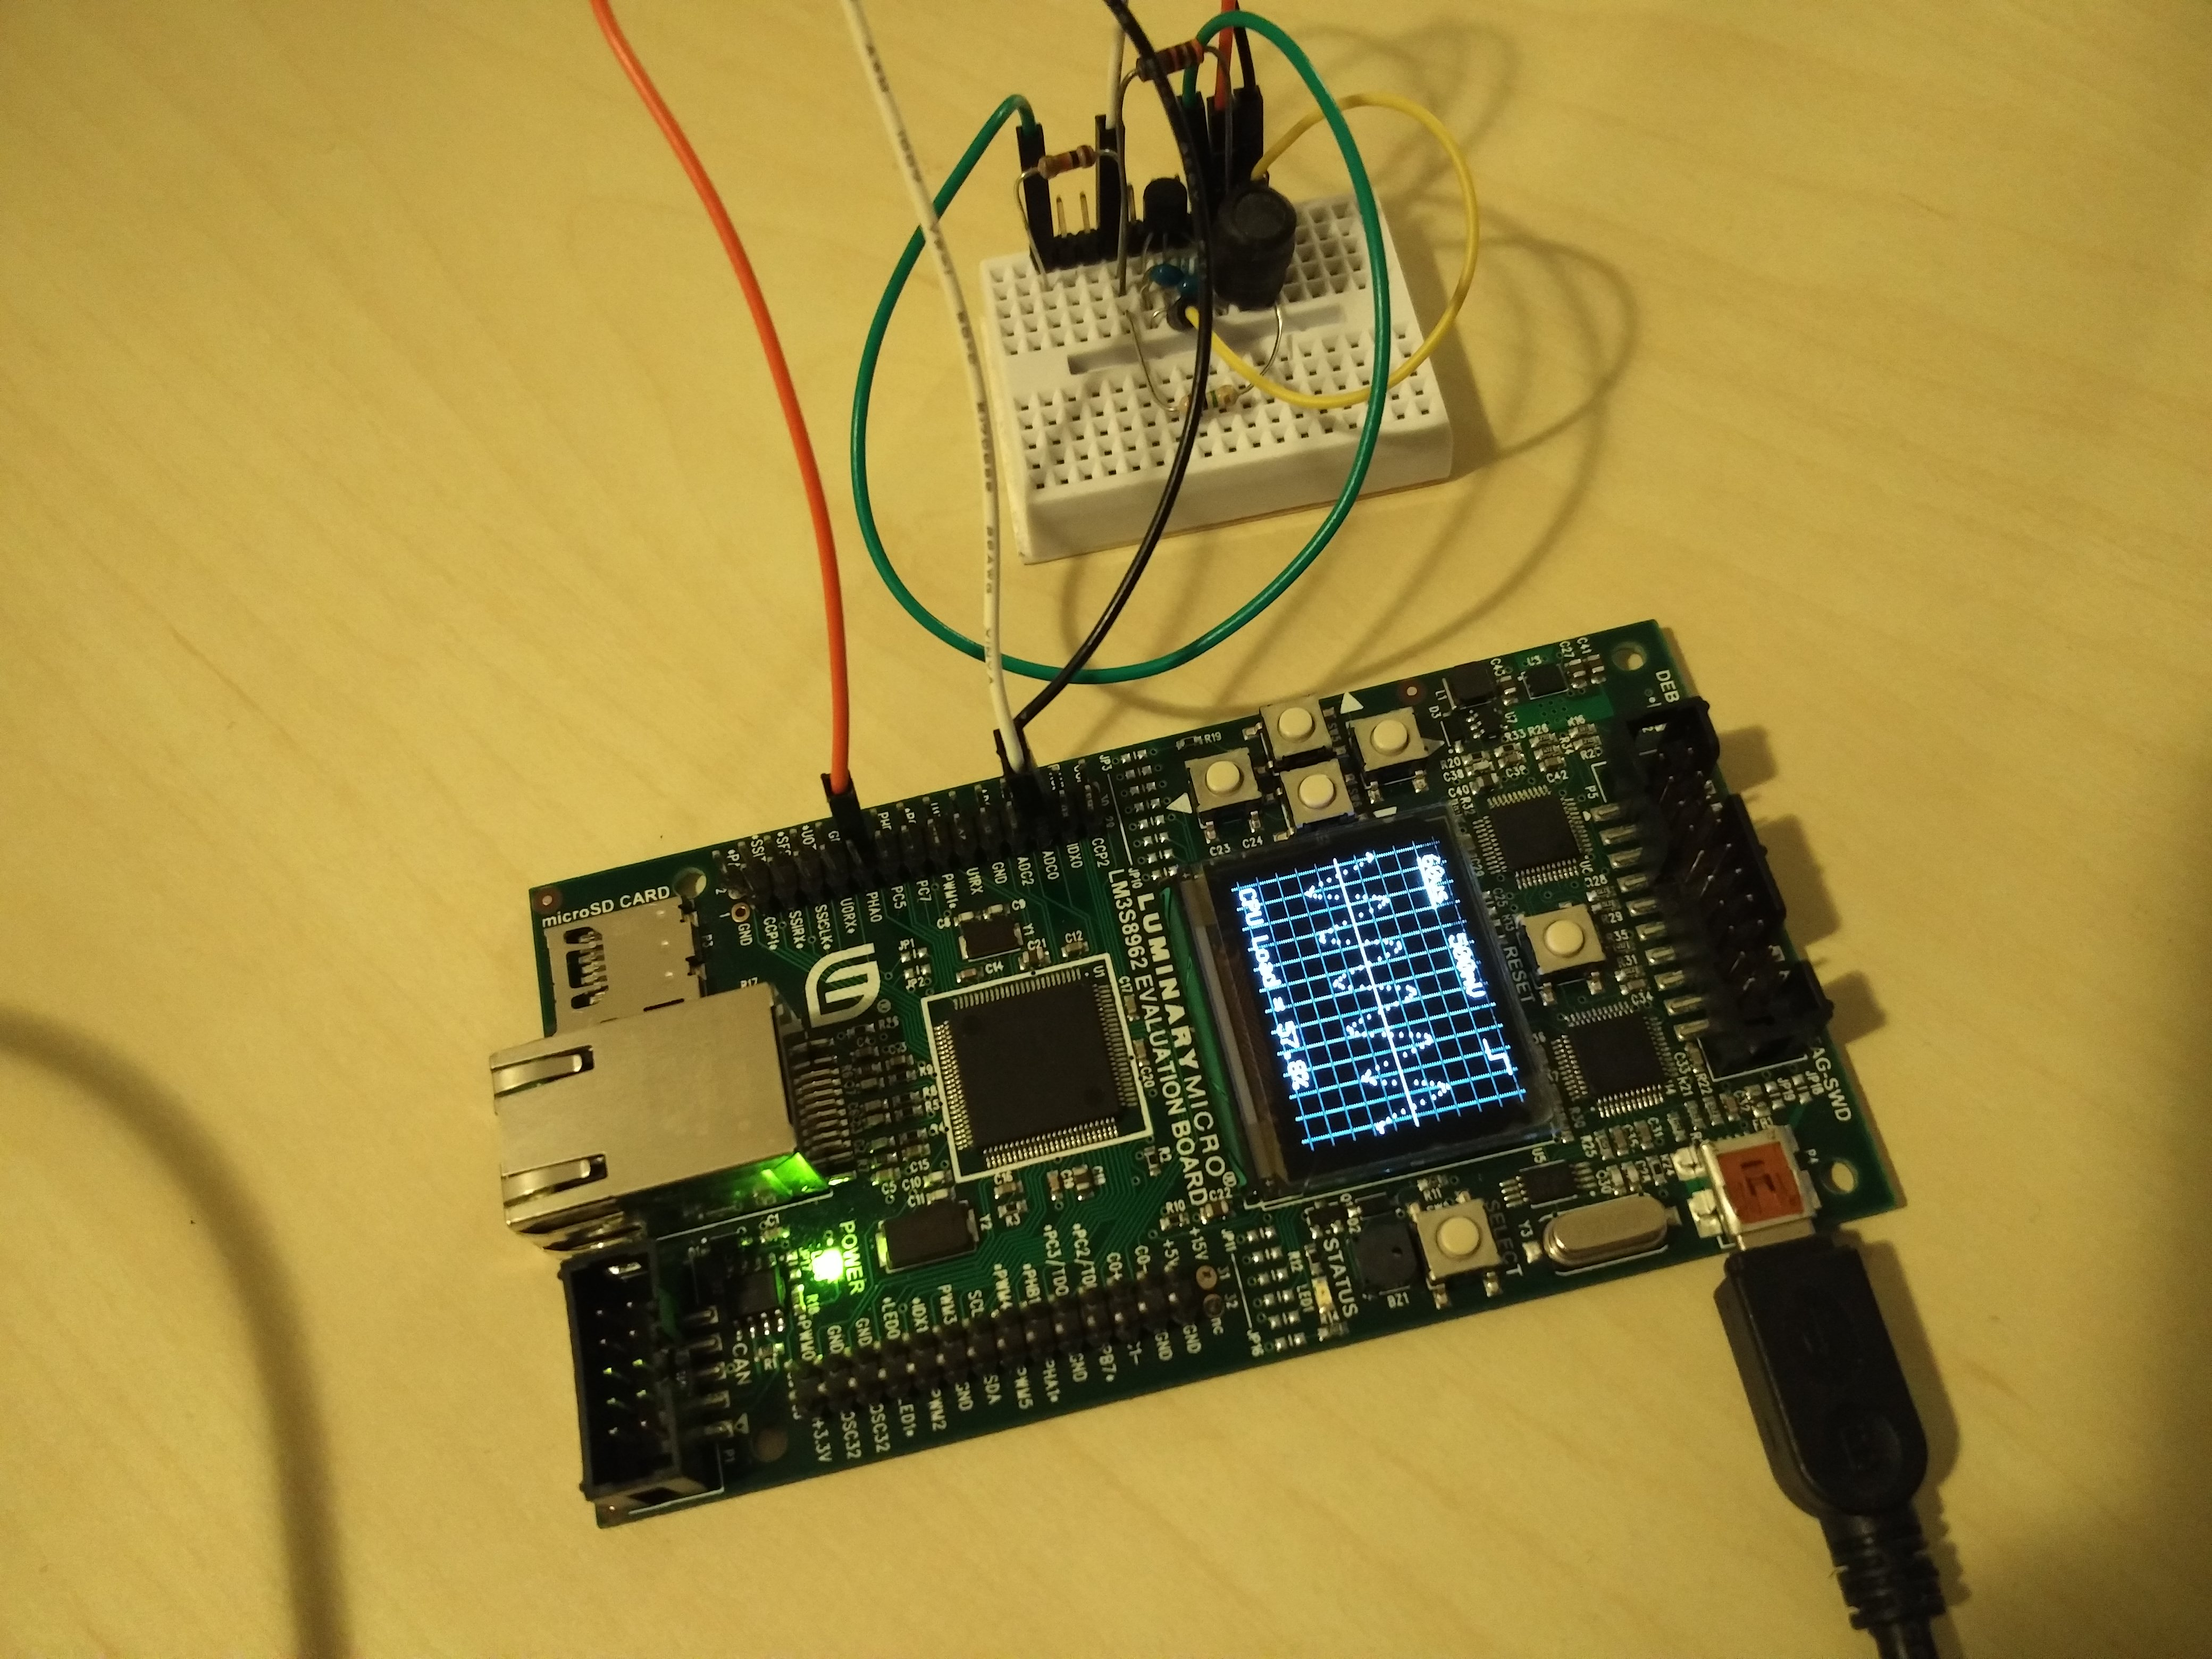
\includegraphics[width=\linewidth]{assets/overview.jpg}
  \caption{Overview of the circuit}
  \label{fig:overview}
\end{figure}

\section{Discussion and Results}
In this part we will discuss the methodologies used during the projects, along with their results.
\begin{figure}[h]
  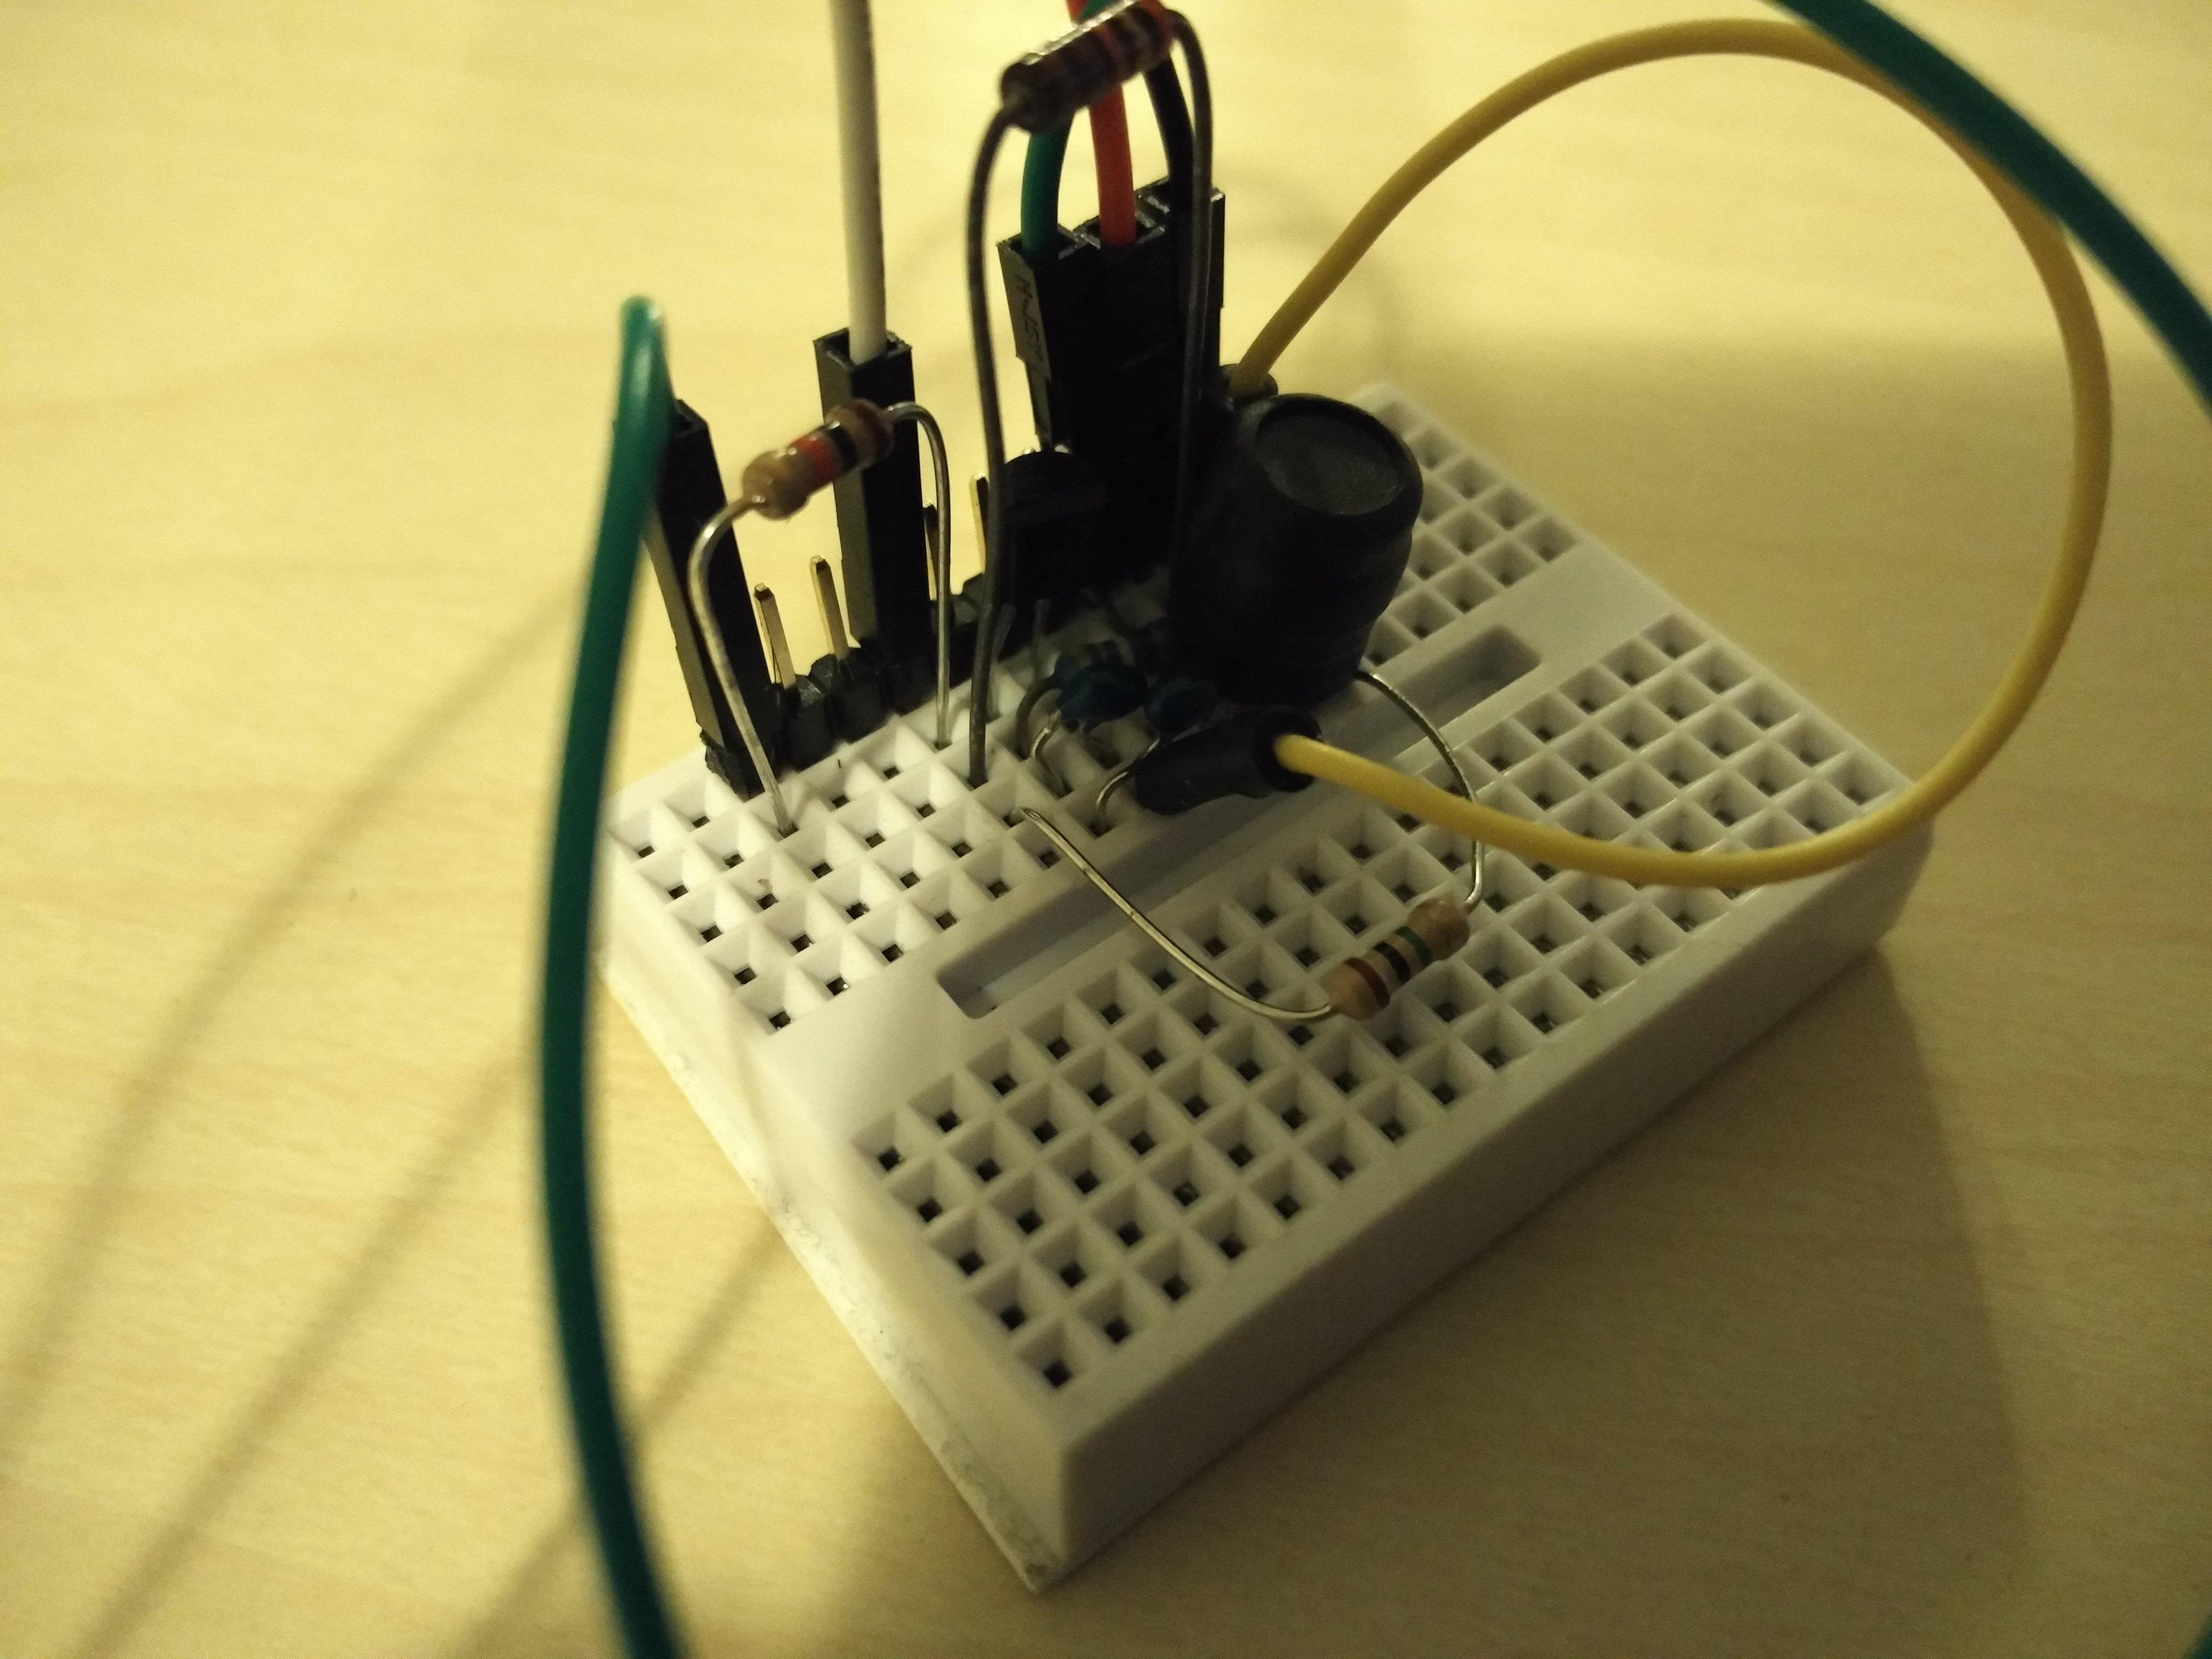
\includegraphics[width=\linewidth]{assets/circuit.jpg}
  \caption{The Colpitts oscillator}
  \label{fig:circuit}
\end{figure}

\subsection{Creating a new SYS/BIOS project}

We started out by creating a new sample SYS/BIOS project, with the basic files to get started and an \texttt{app.cfg}

Before moving on to the project, we configured our debugger to automatically reset the board every time we upload by checking the “Reset target during program load to Flash memory.” option. However, for some unknown reasons, this lead to our board being disconnected from the IDE Debugger. In the end we opted not to use this option, and have not experienced any crashes so far. 

\subsection{Initializing}
Our previous code relied heavily on timers and interrupts to achive real time functionality. Our current task is to replace the previous foreground – background system with an implementation using SYS/BIOS provided functions and features. For this, we first started by going through the code and take out all the timer and interrupt related code. Timers are set by RTOS so our implemetation of timed functions are not recognized. Also RTOS disables all interrupt related functions (except IntMasterEnable and IntMasterDisable), as they would interfeare with RTOS provided real time features. After cleaning, our setup pretty much looked like this:

\lstinputlisting[firstline=123, lastline=132]{assets/main.c}

The timer initialization function is taken out. The button initialization function hasn’t changed at all and the ADC code changed slightly (interrups are taken out) as below.

\subsection{Creating the ADC Hwi}
Next we created an Hwi Object for the ADC, instead of declaring/initializing ISR like Lab 1. We created the Cortex-M3 specific Hwi module, make the priority 0 and the interrupt number as 30 - the interrupt number corresponds to ADC0 on the LM3S8962 board. Then we refer to the \texttt{ADC\_ISR} function by reference.

Declaring the Hwi Object allows us to sample data from the ADC every $2\mu s$, and at priority 0 (highest), the Hwi is zero-latency.

\subsection{Button Scanning}
We then port the button scanning functions to SYS/BIOS. In the last lab, we used timer interrupt to periodically scan the buttons and put them in a buffer array. Since we are using SYS/BIOS, we will be creating a Clock object instead. 

We created a Clock instance with a period of 5ms, following the lab instruction, which then call the \texttt{Button\_Clock} function on every clock tick. 

\lstinputlisting[firstline=396, lastline=403]{assets/main.c}

We also added a flag check for \texttt{displaySignal}, which tells us if Spectrum mode is active or not, and re-render accordingly.

Next, we created three more objects: A Task, for button scanning, A Semaphore, for signaling the button Task, and a Mailbox, for posting button IDs to. We would then have the Button Task looking like this. 

\lstinputlisting[firstline=180, lastline=209]{assets/main.c}

The internal button scanning logic mostly stayed the same, with the addition of a semaphore pending at the beginning of the Task while look, which serves as a blocking call while waiting for the Clock signal. The same pattern can be seen in every other Tasks as well.

\subsection{Creating Task Objects}
We added three more Tasks to the mix, porting over from the last lab, taking care so that shared data is being protected. The three Tasks behave the same as the last lab, however, there was a slight change in each Task with the addition of the new Spectrum mode.

For UserInput\_Task, we added a check for the Select button press, as seen from the Button\_Clock function above. 

\lstinputlisting[firstline=218, lastline=224]{assets/main.c}

For the Display\_Task, we also added a check, drew the Overlay for Spectrum Mode, and draw the transformed data. The decision of using \texttt{DrawPoint} over \texttt{DrawLine} is purely aethestic, as the waveform looks better in our opinions.

\lstinputlisting[firstline=290, lastline=305]{assets/main.c}

Lastly, for the Waveform task, we used the same check to copy the buffer over and redirect the Task to FFT. 
\lstinputlisting[firstline=366, lastline=373]{assets/main.c}

\subsection{Spectrum Mode}
The spectrum mode turned out to be the more straightforward than we initialy thought. The first few lines serve as initialization, as suggested by the lab instruction.

\lstinputlisting[firstline=407, lastline=413]{assets/main.c} 

Then, during the while loop, we convert the data from the buffer to a struct that the KISS\_FFT library can understand, with the imaginary and real portions, which is then fed into the FFT function. Finally, we go through the whole screen width (128 pixels), and fill the data in the display buffer. We are using a separate buffer from the Waveform buffer so that we don't have to recalculate every time we switch back and forth between the two modes. 

\lstinputlisting[firstline=422, lastline=435]{assets/main.c}

Last finishing touches have us change the scale and the offset (currently at $-10$ and $180$, respectively) so that the transformed waveform fits nicely on the screen. Since we opted not to work on the extra credit (partially owe to a lack of sleep), we don't have to worry about accurately scaling the waveform on the screen, although it should not be too hard to calibrate by using the software debugger.

\section{Conclusion}
In this lab we have implemented real time features of a digital oscilloscope using an RTOS distribution SYS/BIOS, running on a Stellaris LM3S8962 microcontroller. The foreground-background system from the previous assignment is completely replaced with the RTOS tasks and shared data objects. We have observed significant increase on the performance and responsiveness of the device, as the CPU usage is now dynamically scaling to 100\% at all times, not wasting any flops available on the system.

\end{document}